%% ========================================================================
%% Latex Template for CSC4006: Research and Development Project
%% Adapted in September 2018 by Dr Blesson Varghese from the IEEE Template
%% School of Electronics, Electrical Engineering and Computer Science
%% Queen's University Belfast, UK
%% ========================================================================


\documentclass[journal]{IEEEtran}
%
% If IEEEtran.cls has not been installed into the LaTeX system files,
% manually specify the path to it like:
% \documentclass[journal]{../sty/IEEEtran}


% Some very useful LaTeX packages include:
% (uncomment the ones you want to load)


% *** MISC UTILITY PACKAGES ***
%
%\usepackage{ifpdf}
% Heiko Oberdiek's ifpdf.sty is very useful if you need conditional
% compilation based on whether the output is pdf or dvi.
% usage:
% \ifpdf
%   % pdf code
% \else
%   % dvi code
% \fi
% The latest version of ifpdf.sty can be obtained from:
% http://www.ctan.org/pkg/ifpdf
% Also, note that IEEEtran.cls V1.7 and later provides a builtin
% \ifCLASSINFOpdf conditional that works the same way.
% When switching from latex to pdflatex and vice-versa, the compiler may
% have to be run twice to clear warning/error messages.





\usepackage{hyperref}

% *** CITATION PACKAGES ***
%
\usepackage{cite}
% cite.sty was written by Donald Arseneau
% V1.6 and later of IEEEtran pre-defines the format of the cite.sty package
% \cite{} output to follow that of the IEEE. Loading the cite package will
% result in citation numbers being automatically sorted and properly
% "compressed/ranged". e.g., [1], [9], [2], [7], [5], [6] without using
% cite.sty will become [1], [2], [5]--[7], [9] using cite.sty. cite.sty's
% \cite will automatically add leading space, if needed. Use cite.sty's
% noadjust option (cite.sty V3.8 and later) if you want to turn this off
% such as if a citation ever needs to be enclosed in parenthesis.
% cite.sty is already installed on most LaTeX systems. Be sure and use
% version 5.0 (2009-03-20) and later if using hyperref.sty.
% The latest version can be obtained at:
% http://www.ctan.org/pkg/cite
% The documentation is contained in the cite.sty file itself.






% *** GRAPHICS RELATED PACKAGES ***
%
\ifCLASSINFOpdf
  \usepackage[pdftex]{graphicx}
  \usepackage{extramarks}
  % declare the path(s) where your graphic files are
  % \graphicspath{{../pdf/}{../jpeg/}}
  % and their extensions so you won't have to specify these with
  % every instance of \includegraphics
  % \DeclareGraphicsExtensions{.pdf,.jpeg,.png}
\else
  % or other class option (dvipsone, dvipdf, if not using dvips). graphicx
  % will default to the driver specified in the system graphics.cfg if no
  % driver is specified.
  % \usepackage[dvips]{graphicx}
  % declare the path(s) where your graphic files are
  % \graphicspath{{../eps/}}
  % and their extensions so you won't have to specify these with
  % every instance of \includegraphics
  % \DeclareGraphicsExtensions{.eps}
\fi
% graphicx was written by David Carlisle and Sebastian Rahtz. It is
% required if you want graphics, photos, etc. graphicx.sty is already
% installed on most LaTeX systems. The latest version and documentation
% can be obtained at: 
% http://www.ctan.org/pkg/graphicx
% Another good source of documentation is "Using Imported Graphics in
% LaTeX2e" by Keith Reckdahl which can be found at:
% http://www.ctan.org/pkg/epslatex
%
% latex, and pdflatex in dvi mode, support graphics in encapsulated
% postscript (.eps) format. pdflatex in pdf mode supports graphics
% in .pdf, .jpeg, .png and .mps (metapost) formats. Users should ensure
% that all non-photo figures use a vector format (.eps, .pdf, .mps) and
% not a bitmapped formats (.jpeg, .png). The IEEE frowns on bitmapped formats
% which can result in "jaggedy"/blurry rendering of lines and letters as
% well as large increases in file sizes.
%
% You can find documentation about the pdfTeX application at:
% http://www.tug.org/applications/pdftex





% *** MATH PACKAGES ***
%
%\usepackage{amsmath}
% A popular package from the American Mathematical Society that provides
% many useful and powerful commands for dealing with mathematics.
%
% Note that the amsmath package sets \interdisplaylinepenalty to 10000
% thus preventing page breaks from occurring within multiline equations. Use:
%\interdisplaylinepenalty=2500
% after loading amsmath to restore such page breaks as IEEEtran.cls normally
% does. amsmath.sty is already installed on most LaTeX systems. The latest
% version and documentation can be obtained at:
% http://www.ctan.org/pkg/amsmath





% *** SPECIALIZED LIST PACKAGES ***
%
%\usepackage{algorithmic}
% algorithmic.sty was written by Peter Williams and Rogerio Brito.
% This package provides an algorithmic environment fo describing algorithms.
% You can use the algorithmic environment in-text or within a figure
% environment to provide for a floating algorithm. Do NOT use the algorithm
% floating environment provided by algorithm.sty (by the same authors) or
% algorithm2e.sty (by Christophe Fiorio) as the IEEE does not use dedicated
% algorithm float types and packages that provide these will not provide
% correct IEEE style captions. The latest version and documentation of
% algorithmic.sty can be obtained at:
% http://www.ctan.org/pkg/algorithms
% Also of interest may be the (relatively newer and more customizable)
% algorithmicx.sty package by Szasz Janos:
% http://www.ctan.org/pkg/algorithmicx




% *** ALIGNMENT PACKAGES ***
%
%\usepackage{array}
% Frank Mittelbach's and David Carlisle's array.sty patches and improves
% the standard LaTeX2e array and tabular environments to provide better
% appearance and additional user controls. As the default LaTeX2e table
% generation code is lacking to the point of almost being broken with
% respect to the quality of the end results, all users are strongly
% advised to use an enhanced (at the very least that provided by array.sty)
% set of table tools. array.sty is already installed on most systems. The
% latest version and documentation can be obtained at:
% http://www.ctan.org/pkg/array


% IEEEtran contains the IEEEeqnarray family of commands that can be used to
% generate multiline equations as well as matrices, tables, etc., of high
% quality.




% *** SUBFIGURE PACKAGES ***
%\ifCLASSOPTIONcompsoc
%  \usepackage[caption=false,font=normalsize,labelfont=sf,textfont=sf]{subfig}
%\else
%  \usepackage[caption=false,font=footnotesize]{subfig}
%\fi
% subfig.sty, written by Steven Douglas Cochran, is the modern replacement
% for subfigure.sty, the latter of which is no longer maintained and is
% incompatible with some LaTeX packages including fixltx2e. However,
% subfig.sty requires and automatically loads Axel Sommerfeldt's caption.sty
% which will override IEEEtran.cls' handling of captions and this will result
% in non-IEEE style figure/table captions. To prevent this problem, be sure
% and invoke subfig.sty's "caption=false" package option (available since
% subfig.sty version 1.3, 2005/06/28) as this is will preserve IEEEtran.cls
% handling of captions.
% Note that the Computer Society format requires a larger sans serif font
% than the serif footnote size font used in traditional IEEE formatting
% and thus the need to invoke different subfig.sty package options depending
% on whether compsoc mode has been enabled.
%
% The latest version and documentation of subfig.sty can be obtained at:
% http://www.ctan.org/pkg/subfig




% *** FLOAT PACKAGES ***
%
%\usepackage{fixltx2e}
% fixltx2e, the successor to the earlier fix2col.sty, was written by
% Frank Mittelbach and David Carlisle. This package corrects a few problems
% in the LaTeX2e kernel, the most notable of which is that in current
% LaTeX2e releases, the ordering of single and double column floats is not
% guaranteed to be preserved. Thus, an unpatched LaTeX2e can allow a
% single column figure to be placed prior to an earlier double column
% figure.
% Be aware that LaTeX2e kernels dated 2015 and later have fixltx2e.sty's
% corrections already built into the system in which case a warning will
% be issued if an attempt is made to load fixltx2e.sty as it is no longer
% needed.
% The latest version and documentation can be found at:
% http://www.ctan.org/pkg/fixltx2e


%\usepackage{stfloats}
% stfloats.sty was written by Sigitas Tolusis. This package gives LaTeX2e
% the ability to do double column floats at the bottom of the page as well
% as the top. (e.g., "\begin{figure*}[!b]" is not normally possible in
% LaTeX2e). It also provides a command:
%\fnbelowfloat
% to enable the placement of footnotes below bottom floats (the standard
% LaTeX2e kernel puts them above bottom floats). This is an invasive package
% which rewrites many portions of the LaTeX2e float routines. It may not work
% with other packages that modify the LaTeX2e float routines. The latest
% version and documentation can be obtained at:
% http://www.ctan.org/pkg/stfloats
% Do not use the stfloats baselinefloat ability as the IEEE does not allow
% \baselineskip to stretch. Authors submitting work to the IEEE should note
% that the IEEE rarely uses double column equations and that authors should try
% to avoid such use. Do not be tempted to use the cuted.sty or midfloat.sty
% packages (also by Sigitas Tolusis) as the IEEE does not format its papers in
% such ways.
% Do not attempt to use stfloats with fixltx2e as they are incompatible.
% Instead, use Morten Hogholm'a dblfloatfix which combines the features
% of both fixltx2e and stfloats:
%
% \usepackage{dblfloatfix}
% The latest version can be found at:
% http://www.ctan.org/pkg/dblfloatfix




%\ifCLASSOPTIONcaptionsoff
%  \usepackage[nomarkers]{endfloat}
% \let\MYoriglatexcaption\caption
% \renewcommand{\caption}[2][\relax]{\MYoriglatexcaption[#2]{#2}}
%\fi
% endfloat.sty was written by James Darrell McCauley, Jeff Goldberg and 
% Axel Sommerfeldt. This package may be useful when used in conjunction with 
% IEEEtran.cls'  captionsoff option. Some IEEE journals/societies require that
% submissions have lists of figures/tables at the end of the paper and that
% figures/tables without any captions are placed on a page by themselves at
% the end of the document. If needed, the draftcls IEEEtran class option or
% \CLASSINPUTbaselinestretch interface can be used to increase the line
% spacing as well. Be sure and use the nomarkers option of endfloat to
% prevent endfloat from "marking" where the figures would have been placed
% in the text. The two hack lines of code above are a slight modification of
% that suggested by in the endfloat docs (section 8.4.1) to ensure that
% the full captions always appear in the list of figures/tables - even if
% the user used the short optional argument of \caption[]{}.
% IEEE papers do not typically make use of \caption[]'s optional argument,
% so this should not be an issue. A similar trick can be used to disable
% captions of packages such as subfig.sty that lack options to turn off
% the subcaptions:
% For subfig.sty:
% \let\MYorigsubfloat\subfloat
% \renewcommand{\subfloat}[2][\relax]{\MYorigsubfloat[]{#2}}
% However, the above trick will not work if both optional arguments of
% the \subfloat command are used. Furthermore, there needs to be a
% description of each subfigure *somewhere* and endfloat does not add
% subfigure captions to its list of figures. Thus, the best approach is to
% avoid the use of subfigure captions (many IEEE journals avoid them anyway)
% and instead reference/explain all the subfigures within the main caption.
% The latest version of endfloat.sty and its documentation can obtained at:
% http://www.ctan.org/pkg/endfloat
%
% The IEEEtran \ifCLASSOPTIONcaptionsoff conditional can also be used
% later in the document, say, to conditionally put the References on a 
% page by themselves.




% *** PDF, URL AND HYPERLINK PACKAGES ***
%
%\usepackage{url}
% url.sty was written by Donald Arseneau. It provides better support for
% handling and breaking URLs. url.sty is already installed on most LaTeX
% systems. The latest version and documentation can be obtained at:
% http://www.ctan.org/pkg/url
% Basically, \url{my_url_here}.




% *** Do not adjust lengths that control margins, column widths, etc. ***
% *** Do not use packages that alter fonts (such as pslatex).         ***
% There should be no need to do such things with IEEEtran.cls V1.6 and later.
% (Unless specifically asked to do so by the journal or conference you plan
% to submit to, of course. )

% Additonal packages
\usepackage{pgfplots}
\usetikzlibrary{
    pgfplots.dateplot,
}

% correct bad hyphenation here
\hyphenation{op-tical net-works semi-conduc-tor}

\NewDocumentCommand{\codeword}{v}{%
    \texttt{\textcolor{blue}{#1}}%
}

\makeatletter % https://tex.stackexchange.com/a/205193/156344
\newcommand*\short[1]{\expandafter\@gobbletwo\number\numexpr#1\relax}
\makeatother

\begin{document}

% Titles are generally capitalized except for words such as a, an, and, as,
% at, but, by, for, in, nor, of, on, or, the, to and up, which are usually
% not capitalized unless they are the first or last word of the title.
% Linebreaks \\ can be used within to get better formatting as desired.
% Do not put math or special symbols in the title.
\title{GitSlice: Slicing the Repository That Feeds Us}

% author names and IEEE memberships
% note positions of commas and nonbreaking spaces ( ~ ) LaTeX will not break
% a structure at a ~ so this keeps an author's name from being broken across
% two lines.
% use \thanks{} to gain access to the first footnote area
% a separate \thanks must be used for each paragraph as LaTeX2e's \thanks
% was not built to handle multiple paragraphs
%
\author{Dylan Wilson \textless\texttt{dwilson402@qub.ac.uk}\textgreater \\ Queen's University Belfast }

\markboth{CSC4006: Research and Development Project}{}%

%If there are multiple Authors
% {Varghese \MakeLowercase{\textit{et al.}}: Template for Research Article}
% The only time the second header will appear is for the odd numbered pages
% after the title page when using the twoside option.
% 
% *** Note that you probably will NOT want to include the author's ***
% *** name in the headers of peer review papers.                   ***
% You can use \ifCLASSOPTIONpeerreview for conditional compilation here if
% you desire.


% make the title area
\maketitle

% As a general rule, do not put math, special symbols or citations
% in the abstract or keywords.
\begin{abstract}
Professional software development teams now almost universally use Git (a distributed version control system) to manage changes to their code.
Git repositories contain metadata relating to the development of the project and show how a project has changed over time.
Analysis of this metadata to gain insight into the software development process is performed in the field of mining software repositories (MSR).
Static code analysis (SCA) tools perform analysis on source code to detect issues during development (they are static because they analyse the code without running it) such as untested or vulnerable code.
SCA only analyses one version of the code, however.
The ability to run code analysis tools across many historic versions of a project could therefore provide useful insight into how the code has changed over time.

A generic approach was implemented to perform iterative execution of SCA tools on historic versions of codebases from Git repositories.
The approach allows for configurable patterns to select commits for analysis.
It is necessary to run the SCA tool in parallel to reduce the time needed to perform analysis, particularly when very large amounts of commits are being analysed.
To demonstrate the utility and flexibility of the approach, a selection of SCA tools were run against popular open source projects to produce time series data showing how the output of these SCA tools changes throughout the evolution of the project.

\end{abstract}

\begin{IEEEkeywords}
Version control systems, Mining software repositories, High-performance computing.
\end{IEEEkeywords}

\IEEEpeerreviewmaketitle

\section{Introduction}
\label{sec:introduction}
Today, virtually all software development teams use version control systems (VCSs) to manage changes in their projects.
StackOverflow reports over 96\% of professional developers use Git~\cite{vcs_usage}.
Git is a distributed VCS developed originally by Linus Torvalds and other contributors to the Linux kernel.
Version control systems enable developers to manage changes to the code in their software projects.

The building block of a Git repository is known as a ``commit''~\cite{pro_git}.
Each commit (except the first) points to one or more commits known as its parent(s) and can be thought of as a set of changes to files which have occurred since its parent commit.
Commits form a tree structure and traversing the tree allows the reconstruction of the filesystem as it existed at that commit.
Multiple commits can have the same parent creating branches.
Commits which have multiple parents are called ``merge commits'' and allow for the changes from one branch to be combined with another.
\autoref{fig:git_branching} shows the Git branching model visually.
In this diagram two branches exist---one at commit \codeword{c2b9e} and another at \codeword{87ab2} which both have \codeword{f30ab} as their parent.

\begin{figure}[ht]
	\centering
	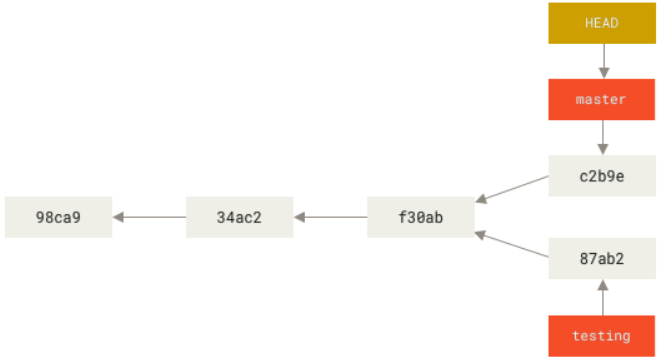
\includegraphics[width=0.475\textwidth]{images/git_branching}
	\caption{Git branching model, two branches exist one called master and one called testing~\cite{pro_git}.}
\label{fig:git_branching}
\end{figure}

Commits contain more information than just changes to file contents---they also include information about who authored the commit and who last applied it (for example, when a commit is imported from a patch file or when the commit is part of a rebase) known as the author and committer respectively.
The field of mining software repositories (MSR) attempts to analyze the contents of software repositories to obtain useful information about a software project~\cite{road_ahead_for_msr}.

Commits are ordered according to their parents.
We can traverse the history of the repository by reversing the changes applied by each commit.
Starting at \codeword{c2b9e} in \autoref{fig:git_branching} the history would contain \codeword{f30ab}, \codeword{34ac2} and \codeword{98ca9} in order of the most recent commits.
Therefore, we can define a window of commits as a subset of all commits in the repository which form a continuous history.
We will traverse this window of commits, and we can apply filter operations to reduce the total amount of commits to be selected based on some metrics (for example files changed, author, time between commits etc.).

Code analysis tools provide various metrics which are used to assess the quality of software code.
Such metrics which may be used include test coverage, and security vulnerabilities.
Tools which do not execute the code but instead analyse the code by reading it are called static code analysis tools.
One common type of static code analysis is static application security testing (SAST).
A SAST tool such a Snyk Code or SonarQube Security Analysis will analyze the code to detect common security vulnerabilities such as the use of known weak hashing or encryption algorithms, or known vulnerable dependency versions~\cite{scat}.
One common limitation of these tools, however, is that they only perform analysis on one version of the software---that is, the version of the software they are provided as they are executed.
Previous versions of the software could still be in use and if a new vulnerability is discovered in a dependency used by older versions of the software, but that version of the dependency is not used by the most recent version of the software, the SAST tool will not identify this vulnerability.
This is a very likely scenario for SAST tools which are constantly updating their vulnerability databases as new vulnerabilities are found and so a scenario where a vulnerability was not known at the time of release but has since been discovered is very likely.

Another example of a code analysis tool is unit test coverage.
This type of tool will run tests written for the software and calculate the percentage of the program tested---often the total lines tested is used but other metrics such as branches taken are also used.
As with SAST tools, code coverage tools only perform analysis on the single version of the software provided to them.
A tool which can perform analysis across different historic versions of the software would enable time series data to be produced to understand how code coverage changes over time.

Iterating through each version of a project sequentially and running analysis can be slow (the Linux repository for example has over 1.3m commits as of Dec 2022 and if each commit only took 1 second to be checked out and analysed it would still take 15 days to go through every commit~\cite{linux_git}).
As each analysis is independent of one another, this problem is very suitable for parallelization which can be used to significantly speed up analysis.
Each process could use an isolated environment to avoid overwriting output from other processes.

Given the common limitation of SCA tools performing analysis on just one version of a software project, a tool called GitSlice has been developed to perform analysis on many versions of a project.
GitSlice allows for a configurable subset of commits in a repository to be selected for analysis using any arbitrary third-party SCA tool.
The analysis tool is run in an isolated environment in parallel and provided with different versions of the project.
The output from this tool is then saved as separate files to an output directory, the names of these files and the output directory are also configurable.
This output can then be used to produce time series data or for further analysis to be performed.


\section{Related Work}
\label{sec:related-work}
GitSlice exists within a field known as Mining Software Repositories (MSR).
Existing approaches in this area were synthesised to understand how these approaches tackled iterating through Git histories.
GitSlice is intended to be used with SCA tools so some existing SCA tools were then researched to identify tools which would potentially be used to validate the approach.
To understand the metrics used by these tools, some time was spent exploring the metrics used by SCA tools.
Finally, as GitSlice needs to perform analysis in parallel, some existing projects which would aid the parallel execution of GitSlice were identified.

\subsection{Mining Software Repositories (MSR)}
\label{subsec:mining-software-repositories-(msr)}

The mining software repositories (MSR) field analyses software repositories to find actionable information about software projects~\cite{msrconf}.
In MSR studies, researchers extract data from a repository to produce evidence to answer a research question~\cite{road_ahead_for_msr}.
While software repositories are typically used as historical records of the software development process, MSR attempts to use the information contained within them to guide future decisions.

Many tools exist to analyse software evolution but these primarily focus on metadata.
For example, one such tool is Boa~\cite{boa} which uses a domain-specific language (DSL) to describe how to mine a selection of software repositories from SourceForge and GitHub.
This enables researchers to write DSL for questions like ``How many files are changed on average per commit in projects which use Java?''.
The tool will then iterate through each commit in every Java project on SourceForge and GitHub to produce the answer.
Boa, however, does not allow for the running of a specific tool on each iteration but rather simply extracting metadata from the commits of the repository.

Similarly to Boa,~\cite{closer} introduces CLOSER which is a DSL for metadata across multiple types of VCSs.
This allows for the conversion of a software repository from one type of VCS to another.
CLOSER primarily focuses on the metadata of a repository (as opposed to each version of code stored within in it) but has provided a starting point for research into this area.

Another example is described in~\cite{libvcs4j} which introduces LibVCS4j, a Java library which enables the mining of software repositories.
LibVCS4j supports multiple types of repository and abstracts the specific VCS away at an API level to enable the mining of data from multiple types of repositories.
Again, however, this library primarily focuses on enabling the mining of metadata from the repository as opposed to performing analysis on the code itself.

\cite{cvsgrab} describes CVSgrab is a tool for visualizing metadata of a CVS repository (an older VCS than Git).
This allows for visualization of different metadata such as the types of files and authors of lines of code.
The tool produces a graph which shows how this metadata changes over time.
CVSgrab however, is built for CVS and doesn't allow the running of any tool on each version of the software but merely one type of visualization of the data contained within the repository.

\cite{mjgit} describes MJgit, a tool which performs code analysis on changes to code in a project by understanding how these changes affect the code.
This allows for better textual search of the source code by ignoring cases where methods were simply moved but their functionality did not change (this would be registered in Git as line deletions then line additions, but wouldn't be included in the search results for MJgit) allowing for more accurate searching of the repository.

The information produced by MSR tools can produce datasets useful to researchers to answer further research questions.
In~\cite{is_refactoring_always_a_good_egg} the authors attempted to understand how commits which refactor code could introduce bugs in the software.
Code refactoring is the process of modifying code while maintaining the same behaviour in attempt to make the code more readable or maintainable.
The authors analysed 96 Java projects in the SmartSHARK dataset to understand how often refactoring commits would induce bugs.
They found that for over half of bug-inducing commits, some refactoring of code was involved.
From this the authors identified the potential for more qualitative research in this area to understand the connection between the refactoring of code and the introduction of bugs.

Another dataset, called World of Code~\cite{world_of_code} provides infrastructure for mining data from open-source repositories.
At the time of publication in 2019, the dataset contained 88 million open-source projects, 1.2 billion commits and 5.5 billion source files.
The purpose of this infrastructure was to provide a dataset for research which depends on measuring interdependencies among projects.
One example of such a research question is given in~\cite{tracing_vulnerable_code_lineage} where the authors developed a tool to show how the duplication of code though the ``forking'' of open-source repositories can cause vulnerabilities to remain even after the vulnerability is fixed in the original source.
They produced a tool which used the World of Code dataset to show how several known vulnerabilities in open source projects RIOT, QEMU and LZ4 had been replicated to other open-source repositories and how these vulnerabilities remained even after the original vulnerability was patched.

MSR can also provide greater societal understanding outside of software development too as the information contained within repositories contains names and email addresses of developers.
In~\cite{geographic_diversity} the authors attempted to answer the question of how the geographic diversity of software contributions has changed over time.
They used multiple methods including analysing email address domain extensions, timezone data and the names of developers to understand how software contributions in 12 geographic regions have changed over time.
They used a very large dataset of 50 years of data containing 2.2 billion commits from 160 million projects.
The authors found that the name Eric, which is descended from Old Norse is more common in Ghana than it is in France or the UK which they understood to be an implication of colonialism and suggested that further research was warranted.

\subsection{Code Quality Metrics}
\label{subsec:code-quality-metrics}

\cite{rosenberg1997software} attempted to identify specific metrics which impact code quality in object-oriented code.
They identified 9 metrics which indicate the codes adherence to the 4 object-oriented principles: methods, cohesion, coupling, and inheritance.

\cite{beck1999bad} popularised the term ``code smells'' which is any properties in code which suggest poor programming techniques.
Importantly, code smells are not bugs and do not cause faults in the application but rather indicate a lack of adherence to common design principles and can indicate that the code may be hard to maintain.
This book highlighted some common factors which may indicate larger problems with the code including large classes, methods or parameters lists and duplicated code among quite a few others.

\cite{6405287} compared common code smells to expert developers subjective options on code.
They asked the developers to assess how maintainable they perceived certain pieces of code to be and scored it using some code smell metrics.
They noted that not all factors that affect code maintainability can be assessed and that more work was necessary to produce an accurate maintainability assessment of a system.

\cite{9463095} introduces QScored, a dataset which contains code quality information in over 86,000 C\# and Java repositories.
Using MSR, the authors produced a dataset which they believe would be useful for research on ``bug prediction, machine learning for software engineering applications and on correlating code quality with effort and productivity''.
The authors suggested this dataset could be improved by expanding to repositories other than C\# and Java however they found an extensive tool support to detect code smells in other languages was lacking.

\cite{7589790} proposed 73 different metrics to access code quality.
The authors then trained an artificial neural network (ANN) to assess files in popular open-source repositories to estimate the quality of the code.
This work suggests that neural networks could prove to be useful in assessing the quality of software code.

\subsection{Source Code Analysis (SCA)}
\label{subsec:source-code-analytics-(sca)}

\cite{1657940} describes static code analysis in Java.
Static code analysis is any form of analysis which assesses code without running it.
One example of this is Lint an early linter, written in C at Bell Labs.
A linter assesses the style of the code based on some predefined rules (for example is might check the length of lines does not exceed a certain threshold).

\cite{sonarqube} compared the features of the three most commonly presented tools for static code analysis in research: Cppcheck, FindBugs and SonarQube.
The finding was of all the features compared, SonarQube provided the greatest feature set.
SonarQube also supports more languages than the other two where Cppcheck only supports C/C++ and FindBugs only supports Java.
Therefore, SonarQube could be used to perform static code analysis on many types of project, and is therefore a good potential candidate for a tool to validate the approach.

\cite{java_ci_sca} investigates the use of static code analysis in the CI/CD pipelines of 20 open-source Java projects.
A majority of projects used a tool called CheckStyle which is a commonly used Java linter.
CheckStyle is another tool which could be used to validate the approach by understanding how rule violations vary over time.
Further, the use of GitSlice in the CI/CD pipeline would enable developers to continually run their static code analysis tools on previous versions of the project.
For example, running GitSlice upon push to a mainline or release branch would ensure older versions are continually checked.

\cite{li_2020} analysed the benefits and limitations of Checkmarx, a common static application security testing (SAST) tool.
This is another good example of the sort of tool which could be used to validate the approach by creating known vulnerable code between specific commits and testing to see if the tool is able to use Checkmarx to find the vulnerability.

Similar to Checkmarx, Semgrep~\cite{semgrep} is a static code analysis tool which supports code quality analysis on Go, Java, JavaScript, JSON, Python and Ruby code.
Semgrep also finds vulnerabilities in dependencies.
Semgrep is one of the static code analysis tools included as part of GitLab's SAST feature.
This is a more modern analysis tool, and it suggests that since~\cite{9463095} in 2012 there has been significant improvement in the development of cross-language static code analysis tools.

Semgrep appears to be the best choice for validating the approach among all the tools listed here for two reasons.
Firstly, CheckMarx is a premium product and Synk Code only permits a certain amount of analyses for free per month.
Secondly, SonarQube publishes its findings to a server, which complicates the setup required.
By contrast Semgrep is free and open-source, and it can generate its findings as terminal output which makes it easier to extract data.

\subsection{Running Repository Mining at Scale}
\label{subsec:running-repository-mining-at-scale}

\cite{torcpy} describes torcpy, a load-balancing Python library which manages the execution of multiple asynchronous tasks and supports OpenMPI which is an open-source MPI implementation that is widely used on computing clusters including Perlmutter, the 8th most powerful supercomputer according to the Nov 2022 TOP500 rankings~\cite{perlmutter}.
This enables multiple versions of the program to run across nodes in a cluster, balancing workload to ensure optimal use of resources.

Some existing work has been done in relation to accessing Git repositories in high-performance computing environments such as RepoFS~\cite{repofs}, a tool for accessing multiple versions of the repository.
RepoFS exposes the commits of the repository as a virtual filesystem, ordered in a tree structure by metadata from the commit by both commit ID and by date of the commit.
Use of RepoFS would allow a highly parallelised analysis to be performed on a shared filesystem against a single copy of a repository rather than making multiple copies each at a specific point.

Running multiple versions of the same program can lead to issues, for example SonarQube will fail to run if another instance is already scanning the same project~\cite{sonarqube_parallel}.
Containers, such as Docker, enable the isolation of a process from the rest of the operating system and ensure that the process will run predictably across different platforms~\cite{container_benefits}.
Running the code analysis tool inside a container also means it will be isolated (including its filesystem) from the other processes on the system allowing for multiple versions of the same tool to run simultaneously without interacting with each other.
An analysis of Docker in high-performance environments shows that it provides performance similar to that of running the software natively (i.e.\ directly on the operating system without any visualisation) and much greater than that of running it inside virtual machines~\cite{docker_hpc}.


\section{Implementation}
\label{sec:implementation}
In order to meet the problem identified in \autoref{sec:introduction}, GitSlice has been implemented as a Python 3 application.
GitSlice is configured using a YAML file, which defines the exact parameters of commits be selected, the analysis tool to be run and the location of output from the analysis tool.
The analysis tool is given as a Singularity image (see \autoref{subsec:singularity}).
GitSlice supports a different analysis tool depending on the version of the project---for example, if a Python project is currently written using Python 3 but a previous version required Python 2, a Python 2 container can be used for older versions.
Similarly, the command to invoke the analysis tool is configurable based on the version---if for example the location of the main script has changed, a command that invokes test coverage may be different depending on the version.

GitSlice can run across multiple nodes in an HPC cluster.
When executed, GitSlice will inspect the repository to identify the commits to be analysed on the primary node (the node with an ID of \codeword{0}) and the commits are then distributed across all the nodes allocated to GitSlice (see \autoref{subsec:mpi}) each of which will begin analysing the commits allocated to it.
Each node will clone the repository and represent it as virtual filesystem, the commit to be analysed will be mounted on the analysis container and the appropriate command (depending on the version) will be run.
GitSlice then presents the files as they existed at that commit to the analysis container by binding the appropriate subdirectory from the virtual filesystem to the container.
The output from the analysis container is then saved to the output directory defined in the configuration file.

\subsection{Parallel Execution using MPI}
\label{subsec:mpi}

GitSlice uses MPI to allow for multiple nodes to work together to analyse the repository.
One instance of GitSlice will be the ``primary'' instance, with $ 0 $ or more ``secondary'' instances which await a commit ID to perform analysis on.
Upon initialisation of GitSlice, the primary instance will analyse the repository to identify the commits to be analysed.
Each instance of GitSlice creates its own directory inside the output directory identified by a UUID generated on initialisation.
This enables any amount of instances of GitSlice to work on analysing the repository without overwriting work from another instance.
The work is evenly divided among all instance of GitSlice---for example, if there are $ 5 $ instances with $ 25 $ commits to be analysed then each instance will analysed $ 5 $ commits.
Multiple threads are also used to allow for each instance to analyse multiple commits simultaneously.
For example, if there are $ 5 $ instances each with $ 5 $ threads then 25 commits will be analysed simultaneously.
\autoref{fig:mpi_diagram} illustrates this visually.

\begin{figure*}[ht]
	\centering
	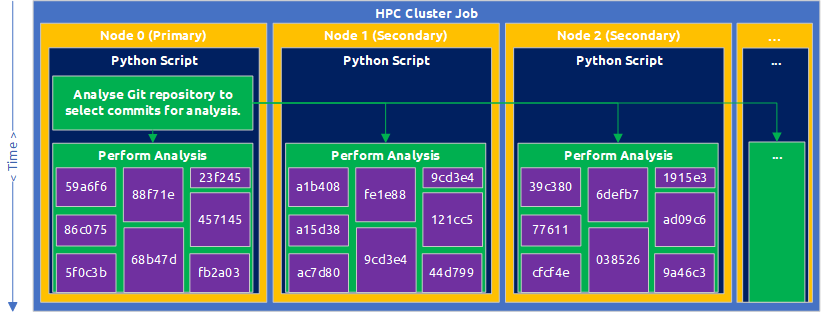
\includegraphics[width=\textwidth]{images/mpi_diagram}
	\caption{Illustration of how GitSlice operates using MPI across multiple nodes.}
\label{fig:mpi_diagram}
\end{figure*}

\subsection{Accessing Git Commits Through a Virtual Filesystem}
\label{subsec:filesystem}

GitSlice needs to recreate the files of the project being analysed as they existed at a particular commit in order to bind this to the analysis container.
Multiple commits cannot be checked out at once so the initial implementation of GitSlice created a copy of the repository for each analysis with the appropriate commit checked out in a detached \codeword{HEAD} state (this means a commit has been checked out directly, as opposed to a branch).
This caused quite a lot of overhead as the entire repository is deleted and copied over and over again.
To prevent this, RepoFS\cite{repofs} was used.
RepoFS is a Python project which exposes the repository as a virtual filesystem.
When run, RepoFS will create a filesystem which contains a directory named \codeword{commits-by-hash/} among others.
Within this directory is a subdirectory for each commit, named using the commit ID of the commit.
Inside each of these commit directories is the project as it existed at that commit.

Each parallel instance mounts its own virtual filesystem as HPC clusters typically use a network filesystem to keep a consistent filesystem across nodes.
Mounts are not shared across the network so each instance must mount its own virtual filesystem.
When an instance is finished analysing all the commits assigned to it, it will bring the mount down.

\subsection{Analysis Using Singularity Containers}
\label{subsec:singularity}

Typically, to run an analysis application it would be necessary to install all the required dependencies which is not an option in HPC cluster environments where installing arbitrary tools is usually not allowed for security reasons.
A solution to this is containers which encapsulate all the required dependencies to run an application within an isolated environment.
Containers utilize the same kernel as their host and in this way they differ from virtual machines---this also makes containers much more lightweight than virtual machines.
Singularity is a container platform designed for use in HPC environments~\cite{singularity}.
It supports Docker images, the most widely used containerisation platform.
Support for Docker images enables a very wide variety of images to be executed, Docker Hub for example currently contains over 100,000 images.

When running an analysis tool, the use of containers also allows for the complete isolation of the filesystem running the analysis tool.
This is important as it prevents multiple executions of an analysis tool from writing to the same files (for example, outputting analysis reports to the same location).

\subsection{Configuration}
\label{subsec:configuration}

When run, GitSlice accepts three arguments; the location of a configuration file, the level of logging to use (where logging output is one of the following: debug, info, warning, error and critical) and if dry run is enabled (in dry run mode GitSlice will not perform analysis but instead will output the commits which would have been selected based on the configuration file).
The configuration file specifies the following settings:

\begin{itemize}
    \item \textbf{Output Directory}: the directory in which the output from each commit will be saved as a text file to.
    \item \textbf{Output Format}: the format of the output file, for example each file can be named by the time of the commit and the commit ID with an underscore to separate them.
          The time of the commit here refers to the commit time as opposed to author time.
          Output files is saved as a .txt file.
    \item \textbf{Temp Directory}: the directory to use for creating a temporary copy of the repository.
          It is recommended this location is stored locally as opposed to a network location for performance.
          It is not necessary for files in the directory to be able to be accessed by all nodes, but all nodes must be able to create directories at this location.
    \item \textbf{Rsync To Temp}: the virtual filesystem is read only so the container cannot modify the or create files.
          GitSlice provides a feature which will use \codeword{rsync} to copy files from the directory containing the files of the commit to be analysed to a temporary directory to enable the analysis tool to modify and create files.
          This feature is enabled when this option is set to true.
    \item \textbf{Mount Directory Name}: the name of the directory inside the temporary directory where the virtual filesystem will be mounted at.
    \item \textbf{Repo Directory Name}: the name of the directory inside the temporary directory which will contain the repository.
    \item \textbf{Git Repository Type}: indicates if the repository is local or remote, remote repositories will be cloned into the temporary directory and local repositories will be copied into it.
    \item \textbf{Git Repository Source}: the source of the repository, an absolute or relative path for local repositories and a full URI for remote repositories.
    \item \textbf{Analysis}: this block contains a list of commits IDs which contain \textbf{Image} and \textbf{Command} values.
          When that commit exists as a parent (not necessarily a direct parent) of the commit, the \textbf{Image} and \textbf{Command} values will be used.
          Where multiple commits listed in this section are parents, the most recent parent's \textbf{Image} and \textbf{Command} values will he used.
    \item \textbf{Starting Point} and \textbf{Stopping Point}: these options provide Git objects (commits, tags, branches etc.) for which the ancestry path between them will be the commits which are selected for analysis.
    \item \textbf{Git Rev List Args}: GitSlice uses the \codeword{git-rev-list} command to find the ancestry between the \textbf{Starting Point} and \textbf{Stopping Point}, this block contains arguments which can be passed to this command.
          This enables a reduction in the commits which are analysed based on a large amount of properties---for example, this allows for selecting only commits created by certain author(s), commits which were committed or authored before or after a certain date, only merge commits to be selected or only non-merge commits to be selected and many more.
          The manual pages for the \codeword{git-rev-list} command provide a thorough explanation of all the options available here.
    \item \textbf{Additional Filters}: finally, GitSlice also provides additional commit filtering options which are not provided by \codeword{git-rev-list}, this includes limiting to a certain amount of commits, skipping a certain amount of commits (for example, select one and then skip 3 commits before selecting the next), selecting only commits with certain amounts of files changed, insertions and deletions, selecting only commits which change particular file types and selecting commits based on a minimum amount of time between commits (i.e.\ one commit every 30 days).
\end{itemize}


\section{Example Application and Evaluation of Approach}
\label{sec:results-and-analysis}
To test the approach outlined in \autoref{sec:implementation}, several third-party SCA tools were selected to perform analysis on several open source projects written multiple languages.
To begin we will use CLOC, a simple Perl script to calculate the total lines of code in a few different popular projects written in Perl, Python and C\@.
We will then use the implementation to perform unit tests in Python and calculate code coverage over time.
Finally, we will look at Semgrep, an SCA tool for detecting bugs and vulnerabilities.

\subsection{Count Lines of Code (CLOC)}
\label{subsec:counting-lines-of-code}

Perhaps the most basic SCA task is to count the lines of code in an application.
Counting lines of code provides a good starting point for assessing the approach.
CLOC (short for count lines of code) is a Perl script which counts the total lines of code across all files in a directory.
It includes breakdowns of programming languages used in a repository.

GitSlice was run using CLOC as the analysis tool against multiple projects written in different languages, specifically CLOC itself, NumPy and Redis.
The output from GitSlice was used to generate time-series data to understand how the total lines of code in an application changes over time.

To start, CLOC was run on its own repository to see how the total lines of code have changed over time in the CLOC script itself.
To collect this data, GitSlice was run on the Kelvin 2 HPC cluster at Queen's University Belfast.
Analysis was run across $ 5 $ nodes on the cluster with $ 5 $ threads per node.

A \codeword{Dockerfile} was written, based on the Perl 5 image from Docker Hub which downloaded the script and saved it as a system command in \codeword{/usr/local/bin}.
This image was built using a GitLab CI/CD pipeline and published to a GitLab container registry.
This image was then pulled by GitSlice and run across all commits in the CLOC repository.
The main branch in the CLOC repository is \codeword{master} so GitSlice was configured to start at the tip of this branch, working backwards through all commits in the repository.

A small Python script was then written to read from the output directory produced by GitSlice, iterating through each of the output files and extracting the total lines of code reported by the CLOC script.
This script works by prompting the user to provide the output directory produced by GitSlice.
It then prompts for some text which should be searched for to find the line containing the value of interest (for example, in this case the text \codeword{SUM:} was used as this line in CLOCs output contains the total lines of code for the application).
Finally, it prompts for the position of the data to extract from the line which matches the search text and searches all text files in the output directory.
This data was saved to a CSV file.

The results are shown in \autoref{fig:cloc_cloc}.
The output from GitSlice shows how the size of the repository has changed significantly over time, growing 5-fold between the start of the project and today.
It also shows how the total lines of code grew significantly in the first year and a half of development and then much more slowly.

\begin{figure}
    \centering
    \begin{tikzpicture}
        \begin{axis}[
            title={Lines of Code in CLOC},
            xlabel={Year},
            ylabel={Total Lines of Code},
            date coordinates in=x,
            xticklabel={\year},
            x tick label style={align=center},
        ]
        \addplot table [
            mark=none, col sep=comma,
            trim cells=true,
            y=LOC
        ] {plots/00-cloc-cloc.csv};
        \end{axis}
    \end{tikzpicture}
    \caption{Graph showing how the total lines of code in CLOC has changed over time.}
    \label{fig:cloc_cloc}
\end{figure}

CLOC is not a particularly active project, currently the repository has only 998 commits and as result all commits were selected for analysis.
It is not always the case that analysis should be run on every commit as it takes time to perform analysis and it may be the case that only the most recent commits are of interest.
NumPy is a much larger project, currently the NumPy repository contains over 32 thousand commits.
NumPy is a Python library which adds support for large multidimensional matrices along with functions to work with them.
It is a very commonly used library in scientific computing such as in physics and mathematics research.

GitSlice allows for the most recent $ x $ commits to be selected.
CLOC was again used to count the line of the code, this time in the NumPy repository but selecting only the $ 5000 $ most recent commits.
GitSlice was run in the same way as before, on the Kelvin 2 HPC cluster across 5 nodes each running 5 tasks.
The same Docker image was used to run CLOC and the same Python script was used to extract data from the GitSlice output.
NumPy uses \codeword{main} instead of \codeword{master} as it's primary branch so GitSlice was configured to use this branch.
CLOC provides more information than just the total lines of code, it also provides a breakdown of how many lines of code have been written in different programming languages.
As GitSlice stores the output directly from the analysis command, all information from the analysis tool is maintained.
In this analysis, the total lines of Python code only were extracted from the output.

The results of this analysis are shown in \autoref{fig:cloc_numpy}.
The output from GitSlice again shows a gradual trend upwards in the total lines of code.
There are some quite significant drops in total lines of code, this is likely caused by refactoring operations.
For example, the most recent drop in commits was caused by the removal of old documentation relating to now non-existent classes and the following commits then added new documentation.

\begin{figure}
    \centering
    \begin{tikzpicture}
        \begin{axis}[
            title={Lines of Code in Numpy},
            xlabel={Year},
            ylabel={Total Lines of Code},
            date coordinates in=x,
            xticklabel={\month/\year},
            x tick label style={align=center},
        ]
        \addplot table [
            mark=none, col sep=comma,
            trim cells=true,
            y=LOC
        ] {plots/01-cloc-numpy.csv};
        \end{axis}
    \end{tikzpicture}
    \caption{Graph showing how the total lines of code in NumPy has changed over time using the main branch as the starting point.  Only the last 5,000 commits were selected for analysis.}
    \label{fig:cloc_numpy}
\end{figure}

Of course, for tasks like counting lines of code it is not necessary to perform analysis on every commit in the repository, as there are likely to be only small differences between commits.
Often, a certain amount of time between commits may be desired.
Redis is a long-running project, first released in 2009 there is over decade of commits in its repository.
Redis is an in-memory key-value store commonly used for caching and session management among other uses.
GitSlice supports selecting only commits which occur after a certain amount of time has passed since the previous commit.
To understand how the total lines of code in Redis has changed since its first release, GitSlice was configured to select one commit every 30 days from the Redis repository.
Aside from limiting commits to one per 30 days, the configuration for GitSlice was otherwise identical to the analysis performed on CLOC and NumPy (i.e.\ it used the same image, same environment with the same amount of resources allocated).
Redis is written in C and so the same Python script as before was used to extract the total lines of C code and the total lines of C/C++ headers.

The results of this analysis are shown in \autoref{fig:cloc_redis}.
As analysis was only performed on one commit each month, a much smoother graph is produced with less sudden variations.
The trend from the previous analyses is shown here too, as the repository ages there is a steady increase in the total lines of code.

\begin{figure}
    \centering
    \begin{tikzpicture}
        \begin{axis}[
            title={Lines of Code in Redis},
            xlabel={Year},
            ylabel={Total Lines of Code},
            date coordinates in=x,
            xticklabel={\year},
            x tick label style={align=center},
            legend pos=north west
        ]
        \addplot table [
            mark=none, col sep=comma,
            trim cells=true,
            y=LOC
        ] {plots/02-cloc-redis-c.csv};
        \addplot table [
            mark=none, col sep=comma,
            trim cells=true,
            y=LOC
        ] {plots/03-cloc-redis-headers.csv};
        \addlegendentry{C Files}
        \addlegendentry{C/C++ Header Files}
        \end{axis}
    \end{tikzpicture}
    \caption{Graph showing how the total lines of code in Redis has changed over time using the unstable branch as the starting point.  One commit every 30 days was selected for analysis.}
    \label{fig:cloc_redis}
\end{figure}

\subsection{Unit Test Coverage}
\label{subsec:unit-tests}

Unit tests are written to confirm the correct functionality of a single piece of code (for example, a single method).
Unit test coverage tools perform SCA to identify lines which are not covered by any tests.
It can be useful to understand how the total amount of code covered by tests in a project changes over time.
GitSlice was again run on the Kelvin 2 HPC cluster to execute the unit tests of the last $ 300 $ commits for the Flask project and find code coverage using Python \codeword{coverage} package.
Flask is a web application framework written in Python, which is commonly used for developing websites and HTTP APIs in Python.

Another \codeword{Dockerfile} was written, based on the Python image from Docker Hub which installed \codeword{rsync} via \codeword{apt-get} which is used by GitSlice for copying the project files to a temporary folder as before running the tests dependencies must be installed and the mounted copy of the project is read-only.
This image was again built using a GitLab CI/CD pipeline and published to a GitLab container registry and pulled by GitSlice.
In the CLOC application the script only needed to be invoked in the directory containing the files, but it is rarely this simple to run a SCA tool as dependencies are often required.
GitSlice was configured to install the dependencies of Flask from PyPi before running the tests to generate code coverage reports.
The main branch in the Flask repository is \codeword{main} and GitSlice was configured to start at this branch.

The results are shown in \autoref{fig:unit-tests-numpy}.
Data was again collecting using the data collection script outlined in \autoref{subsec:counting-lines-of-code}.
The results show a consistently high rate of code coverage, typically above $ 93 $\%.
There is an interesting anomaly around June 2022 caused by commit \codeword{82c2e03} which produced just $ 2\% $ coverage due to a refactor which caused most module imports to fail.
This issue is then fixed in the following commit, \codeword{e0dad45}.
No CI pipeline was performed on \codeword{82c2e03} which suggests it was pushed at the same time as \codeword{e0dad45} which a CI pipeline was run on.
Using GitSlice we are able to identify a bug-inducing commit, given CI never ran for this commit GitSlice has identified a failure which potentially has never been discovered before.

\begin{figure}
    \centering
    \begin{tikzpicture}
        \begin{axis}[
            title={Code coverage (\%) in Flask},
            xlabel={Year},
            ylabel={Code Coverage (\%)},
            date coordinates in=x,
            xticklabel={\month/\short{\year}},
            x tick label style={align=center},
        ]
        \addplot table [
            mark=none,
            col sep=comma,
            trim cells=true,
            y=Coverage
        ] {plots/04-cov-flask.csv};
        \end{axis}
    \end{tikzpicture}
    \caption{Graph showing how the code coverage changes over time on the Flask project.  Analysis was performed on the last $300$ commits on the main branch.}
    \label{fig:unit-tests-numpy}
\end{figure}

\subsection{Static code analysis}
\label{subsec:static-code-analysis}

One of the most common tasks for SCA tools is identifying vulnerabilities.
Semgrep is a static code analysis tool which aims to find vulnerabilities in dependencies, bugs and enforce code standards.
GitSlice can be used to run Semgrep over many versions of a project where Semgrep will usually only perform analysis on one version of the project.
This allows analysis using today's known vulnerabilities against older versions of the project.

As before, GitSlice was run on the Kelvin 2 HPC cluster using 5 nodes each with 5 tasks.
GitSlice was used to perform static code analysis using Semgrep on NumPy which is written in Python.
Often it is not important to perform analysis on every commit, but only every X commit should be analysed.
The commit skip was $ 249 $ meaning every 250th commit on the main branch was analysed.
The ``auto'' configuration was used for Semgrep, this avoids needing to provide a configuration file.

The results are shown in \autoref{fig:semgrep-numpy}.
As before, data was collected using the data collection script outlined in \autoref{subsec:counting-lines-of-code}.
If Semgrep was run when the commits were initially pushed or merged (for example as part of a CI pipeline) then any dependency vulnerability which was not found at the time of the push would not be known.
Using GitSlice allows for each commit to be compared against the most recent vulnerability database and it likely to find more vulnerabilities.
This may be important, especially in such a large project as NumPy which will undoubtedly have many previous versions still in use in projects which have not updated their dependencies.

\begin{figure}
    \centering
    \begin{tikzpicture}
        \begin{axis}[
            title={Total Semgrep findings on NumPy},
            xlabel={Year},
            ylabel={Findings},
            date coordinates in=x,
            xticklabel={\month/\short{\year}},
            x tick label style={align=center},
        ]
            \addplot table [
                mark=none,
                col sep=comma,
                trim cells=true,
                y=Findings
            ] {plots/05-semgrep-numpy.csv};
        \end{axis}
    \end{tikzpicture}
    \caption{Graph showing how the total findings from Semgrep change over time on the NumPy project.  Analysis was performed on every $250$th commit for the last $15,000$ commits on the main branch.}
    \label{fig:semgrep-numpy}
\end{figure}

Semgrep supports a wide variety of languages, not just Python.
GitSlice was run again with the same configuration used for NumPy but this time it was used to perform Semgrep analysis on Jenkins.
Jenkins is an open-source automation server written in Java commonly used to run CI/CD pipelines.
GitSlice supports excluding commits which don't change a particular file type, this analysis was run using only commits which modify \codeword{.java} files.
All other configuration was left exactly the same.

The output from this run is shown in \autoref{fig:semgrep_jenkins}.
This analysis shows a decline in the total findings produced by Semgrep.
Earlier commits appear to have higher findings because of more vulnerabilities discovered in them.
This suggests that GitSlice was able to identify vulnerabilities which would not have been identified when these commits were initially created.

\begin{figure}
    \centering
    \begin{tikzpicture}
        \begin{axis}[
            title={Total Semgrep findings on Jenkins},
            xlabel={Year},
            ylabel={Findings},
            date coordinates in=x,
            xticklabel={\month/\short{\year}},
            x tick label style={align=center},
        ]
            \addplot table [
                mark=none,
                col sep=comma,
                trim cells=true,
                y=findings
            ] {plots/06-semgrep-jenkins.csv};
        \end{axis}
    \end{tikzpicture}
    \caption{Graph showing how the total findings from Semgrep change over time on the Jenkins project.  Analysis was performed on every $10$th commit up to $200$ commits on the main branch.}
    \label{fig:semgrep_jenkins}
\end{figure}


\section{Discussion and Conclusion}
\label{sec:conclusions}
Typically, SCA tools only perform analysis on the version of a project provided to them.
There are scenarios where it may be advantageous to perform analysis again as new information may be available (such as is the case for tools to identify vulnerabilities which have databases which are continually updated).
This is important as older versions of the project may still be in use and as such it would be important to identify vulnerabilities in dependencies for these versions.
Further, it can be useful to generate time-series data to show how metrics of a project have changed over time such a unit test coverage or lines of code.

A generic iterative approach was developed, called GitSlice to enable the execution of any arbitrary SCA tools on historic versions of a software repository.
Results show that this approach was able to perform analysis using multiple third-party SCA tools to perform a variety of common SCA tasks including counting the lines of code, generating unit test coverage and identifying vulnerabilities and bugs.
The projects on which analysis has been performed have been written in multiple languages including Java, Perl, Python and C\@.
The results suggest GitSlice is generic enough to perform analysis using any arbitrary analysis tool and also generic enough to perform analysis independent of project programming language.

GitSlice was configured to initially run a simple script already available in the container but was later configured to install dependencies before running some tests.
This suggests GitSlice is flexible enough to perform analysis which requires some setup tasks such as installing dependencies.
Further, several of GitSlice's commit filtering options were demonstrated including limiting to a certain amount of commits, skipping every $ x $ commits, only selecting commits with more than a certain period of time between them and only selecting commits which modify particular types of files.
Results show these options work well and are able to modify the output produced by GitSlice and significantly speed up execution by avoiding performing analysis on all commits.

Some interesting information was found such as the fact that the projects analysed tend to continually increase in total lines of code as they age and none of the projects tests showed any trend downwards.
GitSlice was able to identify a commit in Flask for which CI was never run and which causes import errors leading to $ 2\% $ code coverage.
Finally, GitSlice was able to show a decrease of findings produced by Semgrep in the Jenkins project, this trend appears to be caused by the fact there is an increase in vulnerabilities for older versions which suggested that GitSlice was able to identify vulnerabilities which were not know originally when the commit was pushed.
Overall GitSlice appears to perform well, and is generic enough to perform many common SCA tasks.

\subsection{Future Work}
\label{subsec:future-work}

One major weakness is that while containerisation has seen significant adoption in software engineering, not all analysis tools will be easily containerised, and it may be easier to run them natively.
This may be the case if a significant amount of dependencies is required and building an image would require very specific dependencies and files to exist in the image.
As a result, GitSlice could be further improved by supporting a native execution option which skips the analysis container and runs the analysis command directly on the host.

Further, \codeword{rsync} is required in an analysis container in order to copy files to a temporary directory where they can be modified.
While this option can be disabled, almost all tools require at least a few files to be created or modified in order to run and \textbf{Rsync To Temp} option (see \autoref{subsec:configuration}) will be required in most situations.
In practice, if it is not possible for \codeword{rsync} to be installed, it is possible for the analysis command to copy the files but this could be supported by GitSlice perhaps by instead using Python's \codeword{shutil.copy()} on the host to create the files in a temporary folder before the analysis container is started.
This would remove the requirement of \codeword{rsync} in the analysis container (which is often not installed to reduce the image size) and mean images could almost always be used directly from popular container repositories such as Docker Hub.

Finally, caching of files used by analysis tools could be improved.
When GitSlice is run, the container is almost completely isolated from the outside which means that files such as build dependencies must be downloaded as part of each analysis.
For large analyses this could cause problems with rate limits where many containers are continually downloading the same files over and over again.
This could be fixed by providing a custom bind mounts option which allows for the configuration file to specify a list of bind mounts for that analysis image.
For example, Maven, a popular Java build automation tool uses a directory \codeword{~/.m2} to cache dependencies it has downloaded, this could be mounted on the container to significantly reduce downloads and speed up execution.


% Can use something like this to put references on a page
% by themselves when using endfloat and the captionsoff option.
\ifCLASSOPTIONcaptionsoff
  \newpage
\fi

% trigger a \newpage just before the given reference
% number - used to balance the columns on the last page
% adjust value as needed - may need to be readjusted if
% the document is modified later
%\IEEEtriggeratref{8}
% The "triggered" command can be changed if desired:
%\IEEEtriggercmd{\enlargethispage{-5in}}

% references section

% can use a bibliography generated by BibTeX as a .bbl file
% BibTeX documentation can be easily obtained at:
% http://mirror.ctan.org/biblio/bibtex/contrib/doc/
% The IEEEtran BibTeX style support page is at:
% http://www.michaelshell.org/tex/ieeetran/bibtex/
%\bibliographystyle{IEEEtran}
% argument is your BibTeX string definitions and bibliography database(s)
%\bibliography{IEEEabrv,../bib/paper}
%
% <OR> manually copy in the resultant .bbl file
% set second argument of \begin to the number of references
% (used to reserve space for the reference number labels box)
\bibliographystyle{IEEEtran}  
\bibliography{references}


% that's all folks
\end{document}


